\subsection*{Functions as Relations}
% Define functions as associations between sets and as relations.
\begin{defn}[Function]
    A \emph{function} is a relation between two sets, the first called the \emph{domain} and the second the \emph{codomain}, such that for each \(x\) in the domain there is {\em exactly} one \(y\) in the codomain associated with \(x\).  Further, the set of all \(y\) from the codomain which are associated with at least one \(x\) in the domain is called the \emph{range}.
\end{defn}


% Domain, Co-Domain, Range/Image


\begin{expository}[sidebyside,sidebyside align=top]{Function Example}
    Define a function \(f\) from the Domain \[D=\{a,b,c,d\}\] to the Codomain \[C=\{1,2,3,4,5\}\] with the following set of pairs:
    \[f=\left\{(a,3),(b,4),(c,2),(d,5)\right\}.\]
    Since there are no letters associated with the \(1\in C\), the Range is
    \begin{align*}
        R&=\{y\in C|\exists x\in D \wedge f(x)=y\}\\
            &=\{2,3,4,5\}.
    \end{align*}
\tcblower
    \centering
    \begin{tikzpicture}[node distance=0.5cm]
    % Sets
        \draw (0,-2.25) ellipse (1cm and 2.25cm);
        \node (a) at (0,-0.75) {\(a\)};
        \node (b) [below=of a] {\(b\)};
        \node (c) [below=of b] {\(c\)};
        \node (d) [below=of c] {\(d\)};
        \draw (4,-2.75) ellipse (1cm and 3cm);
        \node (1) at (4,-0.5) {\(1\)};
        \node (2) [below=of 1] {\(2\)};
        \node (3) [below=of 2] {\(3\)};
        \node (4) [below=of 3] {\(4\)};
        \node (5) [below=of 4] {\(5\)};
    % Function
    \foreach \x/\y in {a/3,b/4,c/2,d/5}{
        \draw[line width=3pt,background] (\x) -- (\y);
        \draw[->,thick] (\x) -- (\y);
    }
    % Labels
        \node at (0,1) {\(Domain\)};
        \node at (4,1) {\(Codomain\)};
        \draw[
            decorate,decoration={brace,amplitude=10pt},
            secondaryaccent,ultra thick
        ] (4.25,-1.125) -- (4.25,-5) 
            node[
                anchor=south,pos=0.35,right,sloped,yshift=20pt,fill=background,rounded corners
            ]{\(Range\)};
    \end{tikzpicture}
\end{expository}

% Exmaple given set draw diagram
\begin{practice}[sidebyside,sidebyside align=top]{Set to Diagram}
    Define a function \(S\) from the Primes \[P=\{2,3,5,7,11,\ldots\}\] to the Alphabet \[A=\{a,b,c,d,e,\ldots,w,x,y,z\}\] with the following set of pairs:
    \[S=\left\{(2,w),(3,h),(5,i),(7,e),(11,l),\ldots\right\}.\]
\tcblower
    \centering
    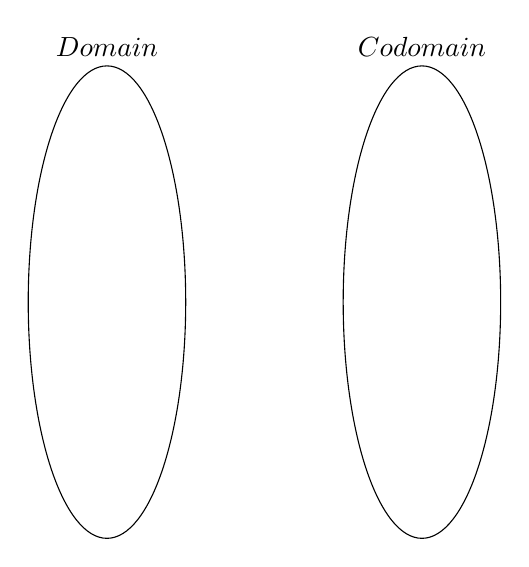
\begin{tikzpicture}[node distance=0.5]
    % Sets
        \draw (0,0) ellipse (1cm and 3cm);
        \draw (4,0) ellipse (1cm and 3cm);
    % Function
    % Labels
        \node[anchor=south] at (0,3) {\(Domain\)};
        \node[anchor=south] at (4,3) {\(Codomain\)};
    \end{tikzpicture}
\end{practice}

\clearpage

% Example given diagram give set of pairs

\begin{practice}[sidebyside,sidebyside align=top]{Diagram to Set}
    What ordered pairs are in the function illustrated on the right?\vspace{5\baselineskip}

    What is the range of the illustrated function?
\tcblower
    \centering
    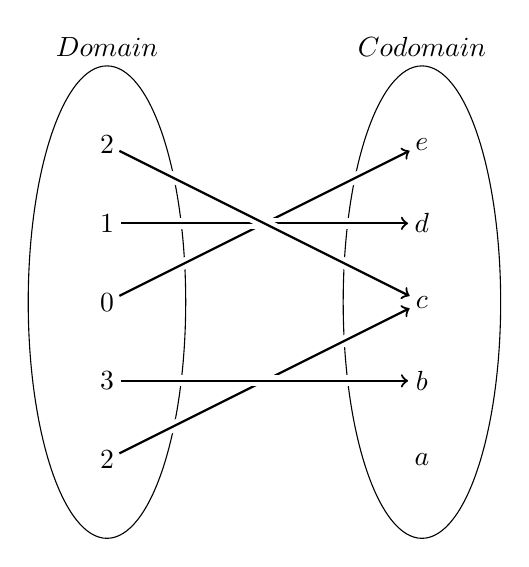
\begin{tikzpicture}[node distance=0.5]
    % Sets
        % Domain
        \draw (0,0) ellipse (1cm and 3cm);
        % Codomain
        \draw (4,0) ellipse (1cm and 3cm);
    % Function
        \foreach \x/\c in {-2/a,-1/b,0/c,1/d,2/e}{
            \pgfmathparse{int(Mod(\x,4))}\let\y=\pgfmathresult;
            \draw[->,line width=4pt,shorten <=5pt,shorten >=5pt,white] (0,\x) -- (4,2-\y);
            \draw[->,thick,shorten <=5pt,shorten >=5pt] (0,\x) node {\y} -- (4,2-\y);
            \node at (4,\x) {\(\c\)};
        }
    % Labels
        \node[anchor=south] at (0,3) {\(Domain\)};
        \node[anchor=south] at (4,3) {\(Codomain\)};
    \end{tikzpicture}
\end{practice}

% Example to discuss function Notation

\begin{practice}[sidebyside,sidebyside align=top]{Function Notation}
    Define
    \begin{equation*}
        P(x)=
        \left\{
            \begin{array}{ll}
                0 & if\ x\ is\ not\ prime \\
                1 &  if\ x\ is\ prime
            \end{array}
        \right.
    \end{equation*}
    Evaluate the function at each point in the domain \[D=\{1,2,3,5,6,7,8,9,10\}.\]
\tcblower
    \centering
    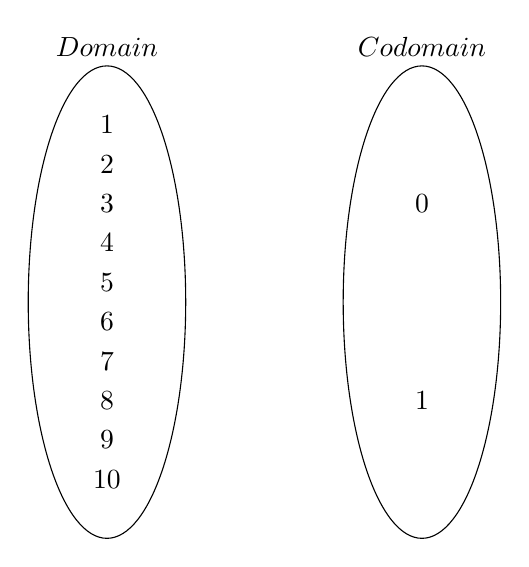
\begin{tikzpicture}[node distance=0.5]
    % Sets
        \draw (0,0) ellipse (1cm and 3cm);
        \foreach \n in {1,...,10}{
            \node at (0,2.75-\n/2) {\n};
        }
        \draw (4,0) ellipse (1cm and 3cm);
        \node at (4,1.25) {0};
        \node at (4,-1.25) {1};
    % Function
    % Labels
        \node[anchor=south] at (0,3) {\(Domain\)};
        \node[anchor=south] at (4,3) {\(Codomain\)};
    \end{tikzpicture}
\end{practice}

% Example to discuss function Notation

\begin{practice}[sidebyside,sidebyside align=top]{Function Notation}
    Define
    \begin{equation*}
        S(x) = 1/\sqrt{x^2+1}
    \end{equation*}
    Evaluate the function at selection of points in the domain \[D=(-4,4)\subset\bbR.\]
\tcblower
    \centering
    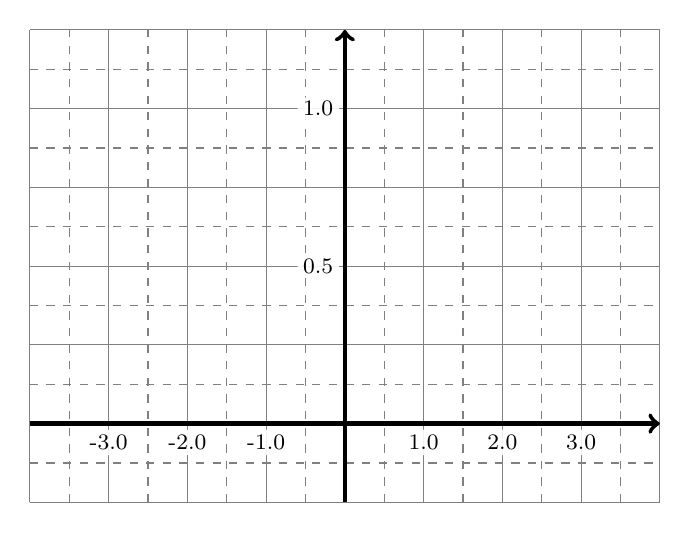
\begin{tikzpicture}[
            every node/.style={
                fill=white,rectangle,inner sep=2pt,
                fill opacity=0.9,text opacity=1,rounded corners=5pt,rounded corners=5pt,
                font=\footnotesize
            },
            scale=1
        ]    
    % Sets
        \draw[step=0.5,gray,dashed,thin] (-4,-3) grid (4,3);
        \draw[gray] (-4,-3) grid (4,3);
        \draw[->,ultra thick] (-4,-2) -- (4,-2);
        \draw[->,ultra thick] (0,-3) -- (0,3);
    % Function
    % Labels
        \node[anchor=east,xshift=-2pt] at (0,2) {1.0};
        \node[anchor=east,xshift=-2pt] at (0,0) {0.5};
    \foreach\x in {-3.0,-2.0,-1.0,1.0,2.0,3.0}{
        \node[anchor=north,yshift=-2pt] at (\x,-2) {\x};
    }
    \end{tikzpicture}
\end{practice}

\clearpage

\subsection*{Properties of Functions}

\begin{defn}[Properties of Functions]
    A function \(f:A\longrightarrow B\) is said to be \emph{one-to-one} (\(1-1\)) if for all \(y\) in the range there is exactly one \(x\) in the domain such that \(f(x)=y\).  The function is \emph{onto} if for all \(y\) in the codomain there is at least one \(x\) in the domain such that \(f(x)=y\).  If a function is both one-to-one and onto we say that it is a \emph{bijection}.
    \begin{itemize}
        \item One-to-One: \(\forall x_0,x_1\in A: f(x_0)=f(x_1) \longrightarrow x_0=x_1\)
        \item Onto: \(\forall y\in B\, \exists x\in A: f(x)=y\)
    \end{itemize}
\end{defn}

% One-to-One, Onto, Bijections

\begin{practice}[label=tcb:maps]{One-to-One, Onto, and Bijections}
    Label each as 1-1, onto, both, or neither.
    \begin{tcolorbox}[sidebyside,colback=white,frame empty]
    \centering
        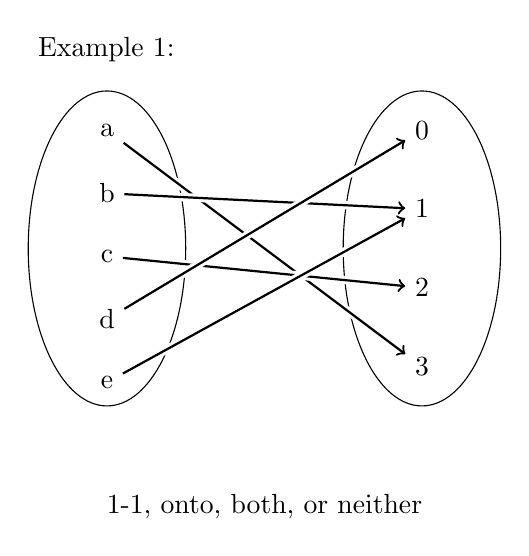
\begin{tikzpicture}
        % sets
            \draw (0,0) ellipse (1cm and 2cm);
            \draw (4,0) ellipse (1cm and 2cm);
            \foreach \y/\v in {0/a,1/b,2/c,3/d,4/e}{
                \node (\v) at (0,1.5-4/5*\y) {\v};
            }
            \foreach \y/\v in {0,1,2,3}{
                \node (\y) at (4,1.5-\y) {\y};
            }
        % function
            \foreach \y/\v in {3/a,1/b,2/c,0/d,1/e}{
                \draw[line width=3pt, white] (\v) -- (\y);            
                \draw[->,thick] (\v) -- (\y);
            }
        % labels
            \node[anchor=south west] at (-1,2.25) {Example 1:};
            \node[anchor=north] at (2,-3) {1-1, onto, both, or neither};
        \end{tikzpicture}\vspace{2\baselineskip}

        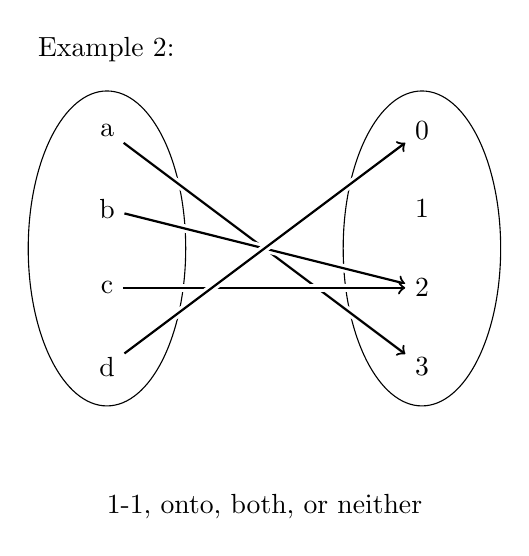
\begin{tikzpicture}
        % sets
            \draw (0,0) ellipse (1cm and 2cm);
            \draw (4,0) ellipse (1cm and 2cm);
            \foreach \y/\v in {0/a,1/b,2/c,3/d}{
                \node (\v) at (0,1.5-\y) {\v};
                \node (\y) at (4,1.5-\y) {\y};
            }
        % function
            \foreach \y/\v in {3/a,2/b,2/c,0/d}{
                \draw[line width=3pt, white] (\v) -- (\y);            
                \draw[->,thick] (\v) -- (\y);
            }
        % labels
            \node[anchor=south west] at (-1,2.25) {Example 2:};
            \node[anchor=north] at (2,-3) {1-1, onto, both, or neither};
        \end{tikzpicture}\vspace{2\baselineskip}

    \tcblower
    \centering

        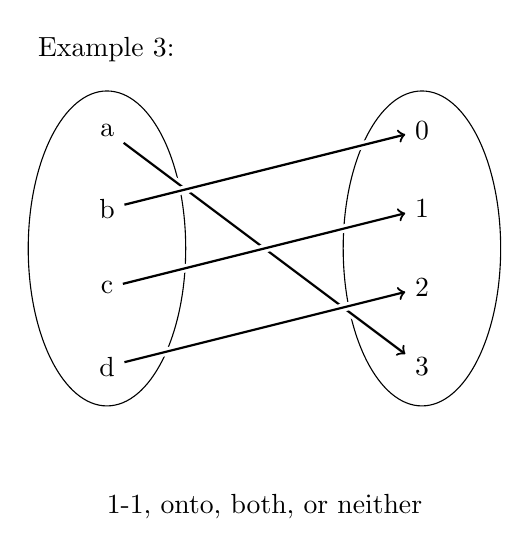
\begin{tikzpicture}
        % sets
            \draw (0,0) ellipse (1cm and 2cm);
            \draw (4,0) ellipse (1cm and 2cm);
            \foreach \y/\v in {0/a,1/b,2/c,3/d}{
                \node (\v) at (0,1.5-\y) {\v};
                \node (\y) at (4,1.5-\y) {\y};
            }
        % function
            \foreach \y/\v in {3/a,0/b,1/c,2/d}{
                \draw[line width=3pt, white] (\v) -- (\y);            
                \draw[->,thick] (\v) -- (\y);
            }
        % labels
            \node[anchor=south west] at (-1,2.25) {Example 3:};
            \node[anchor=north] at (2,-3) {1-1, onto, both, or neither};
        \end{tikzpicture}\vspace{2\baselineskip}
        
        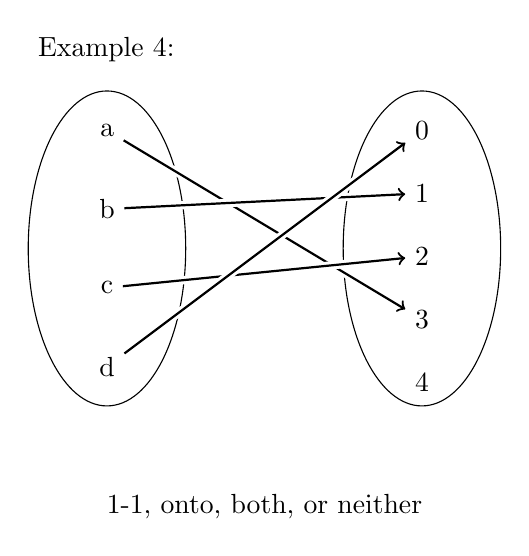
\begin{tikzpicture}
        % sets
            \draw (0,0) ellipse (1cm and 2cm);
            \draw (4,0) ellipse (1cm and 2cm);
            \foreach \y/\v in {0/a,1/b,2/c,3/d}{
                \node (\v) at (0,1.5-\y) {\v};
            }
            \foreach \y/\v in {0,1,2,3,4}{
                \node (\y) at (4,1.5-4/5*\y) {\y};
            }
        % function
            \foreach \y/\v in {3/a,1/b,2/c,0/d}{
                \draw[line width=3pt, white] (\v) -- (\y);            
                \draw[->,thick] (\v) -- (\y);
            }
        % labels
            \node[anchor=south west] at (-1,2.25) {Example 4:};
            \node[anchor=north] at (2,-3) {1-1, onto, both, or neither};
        \end{tikzpicture}\vspace{2\baselineskip}
    \end{tcolorbox}
\end{practice}

\clearpage

\begin{practice}{A Subtle Example}
Is the below function 1-1, onto, both, or neither?  The answer depends on the {\em domain} and {\em codomain}.  For each description, let \(S\) be the set of points on the spiral.

    \begin{tcolorbox}[sidebyside,colback=white,frame empty]
    \centering
        \begin{tikzpicture}[
                every node/.style={
                    fill=white,rectangle,inner sep=2pt,
                    fill opacity=0.9,text opacity=1,rounded corners=5pt,rounded corners=5pt,
                    font=\footnotesize
                },
                scale=0.9
            ]
        % Axes
            \draw[step=0.5,gray,dashed,thin,opacity=0.5] (-4,-4) grid (4,4);
            \draw[gray,opacity=0.5] (-4,-4) grid (4,4);
            \draw[->,ultra thick] (-4,0) -- (4,0) node[anchor=west] {\(x\)};
            \draw[->,ultra thick] (0,-4) -- (0,4) node[anchor=south] {\(y\)};
        % Labels
        \foreach\x in {-3,-2,-1,1,2,3}{
            \node[anchor=north,yshift=-2pt] at (\x,0) {\x};
            \node[anchor=east,xshift=-2pt] at (0,\x) {\x};
        }
        % Function
            \draw[variable=\t,domain=0:1200,->,samples=200,ultra thick,secondaryaccent] plot({\t/360*cos(\t)},{\t/360*sin(\t)});
        % function labels
            \coordinate (s) at (60:1140/360);
            \coordinate (sx) at (0:{1140/360*cos(60)});
            \draw[accent,dashed,thick] (0,0) -- (s) -- (sx);
            \shade[ball color=accent] (s) circle (3pt) node[anchor=south west,xshift=2pt] {\(s=(x,y)\)};
            \draw[dashed,accent,thick] (0:0.5) arc (0:60:0.5) node[pos=0.5,anchor=south west]{\(t\)};
        \end{tikzpicture}
    \tcblower 
    \begin{enumerate}
        \item {\em Domain:} \(\bbR\), {\em Codomain} \(\bbR\): \[f(x)=y,\ \text{if \((x,y)\in S\)}.\] 
        \item {\em Domain:} \(\bbR\), {\em Codomain} \(\mathscr{P}(\bbR)\): \[f(x)=\left\{y\middle|(x,y)\in S\right\}\]
        \item {\em Domain:} \(\bbR^+\), {\em Codomain} \(\bbR\times \bbR\):
            \[f(t)=\left<\frac{t}{2\pi}\cdot\cos(t),\frac{t}{2\pi}\cdot\sin(t)\right>\]
        \item {\em Domain:} \(S\), {\em Codomain} \(\bbR^+\): for \(s\in S\)
            \[f(s)=\text{length of the spiral up to \(s\)}\]
    \end{enumerate}
    \end{tcolorbox}
\end{practice}

\begin{defn}[Inverses]
    Given a relation \(R\) define the \emph{inverse} of \(R\) to be the set \[R^{-1}=\left\{(y,x)\middle|(x,y)\in R\right\}.\]
    If \(R\) and \(R^{-1}\) are also functions, then we say \(R\) is \emph{inevitable}.
\end{defn}

\begin{practice}{Invertible?}
    For each function in practice block \ref{tcb:maps}, write the function and its ``inverse'' as sets of ordered pairs \(R\) and \(R^{-1}\).  Which functions are invertible?  What other property do all those functions have?
    \begin{itemize}
    \foreach \exmp in {1,...,4}{
        \item[]Example \exmp:\vspace{0.9\baselineskip}
    }
    \end{itemize}
\end{practice}

\begin{thm}[Invertible Functions]
    A function will be invertible if and only if it is \hrulefill\phantom{\rule{0pt}{20pt}} 
\end{thm}

\clearpage

% Composing Functions

\begin{defn}
    Given a function \(f:A\rightarrow B\) and \(g:B\rightarrow C\), the \emph{composition} of \(f\) and \(g\) is a function from the domain of \(f\) to the codomain of \(g\) defined by \(g\circ f(x)=g(f(x))\) and we read \(g\circ f\) as ``\(g\) compose \(f\).''
    \begin{center}
        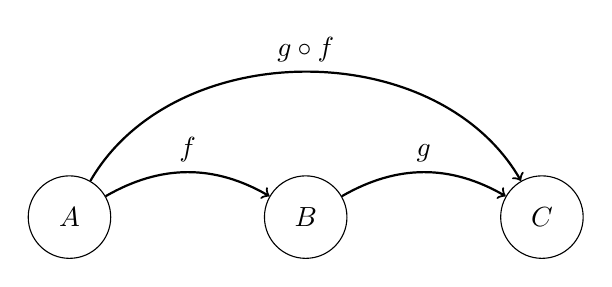
\begin{tikzpicture}
        % Sets
            \node[draw, circle, text width=20pt,align=center] (A) at (0,0) {\(A\)};
            \node[draw, circle, text width=20pt,align=center] (B) at (3,0) {\(B\)};
            \node[draw, circle, text width=20pt,align=center] (C) at (6,0) {\(C\)};
        % Functions
            \draw[->,thick] (A) to[bend left] node[pos=0.5,above] {\(f\)} (B);
            \draw[->,thick] (B) to[bend left] node[pos=0.5,above] {\(g\)} (C);
            \draw[->,thick,bend angle=60] (A) to[bend left] node[pos=0.5,above] {\(g\circ f\)} (C);
        \end{tikzpicture}
    \end{center}
    Note, this is well defined as long as the range of \(f\) is a subset of the domain of \(g\).
\end{defn}

\begin{practice}[]{Composing Functions}
    Is \(g\circ f(x)\)\  1-1, onto, both, or neither?  How does this compare to \(f\) and \(g\) individually?
    \begin{tcolorbox}[sidebyside,colback=white,frame empty]
    \centering
        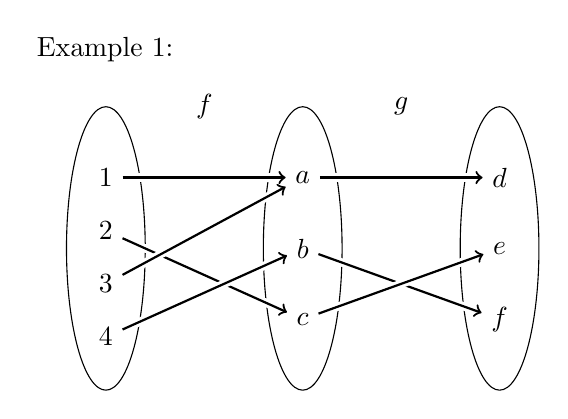
\begin{tikzpicture}[yscale=0.9]
        % sets
            \draw (0,0) ellipse (0.5cm and 2cm);
            \draw (2.5,0) ellipse (0.5cm and 2cm);
            \draw (5,0) ellipse (0.5cm and 2cm);
            \foreach \y/\a/\b/\c in {0/1/a/d,1/2/b/e,2/3/c/f}{
                \node (\a) at (0,1-3/4*\y) {\(\a\)}; 
                \node (\b) at (2.5,1-\y) {\(\b\)}; 
                \node (\c) at (5,1-\y) {\(\c\)}; 
            }
                \node (4) at (0,1-3/4*3) {\(4\)}; 
        % function
            \foreach \a/\b in {1/a,2/c,3/a,4/b}{
                \draw[line width=3pt, white] (\a) -- (\b);            
                \draw[->,thick] (\a) -- (\b);
            }
            \foreach \b/\c in {a/d,b/f,c/e}{
                \draw[line width=3pt, white] (\b) -- (\c);            
                \draw[->,thick] (\b) -- (\c);
            }
        % labels
            \node[anchor=south west] at (-1,2.5) {Example 1:};
            \node at (1.25,2) {\(f\)};
            \node at (3.75,2) {\(g\)};
        \end{tikzpicture}\vspace{\baselineskip}

        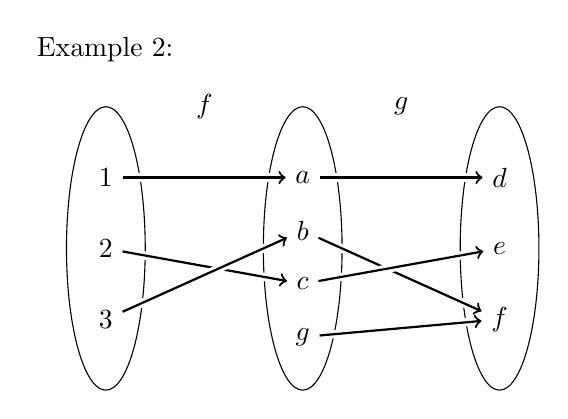
\begin{tikzpicture}[yscale=0.9]
        % sets
            \draw (0,0) ellipse (0.5cm and 2cm);
            \draw (2.5,0) ellipse (0.5cm and 2cm);
            \draw (5,0) ellipse (0.5cm and 2cm);
            \foreach \y/\a/\b/\c in {0/1/a/d,1/2/b/e,2/3/c/f}{
                \node (\a) at (0,1-\y) {\(\a\)}; 
                \node (\b) at (2.5,1-3/4*\y) {\(\b\)}; 
                \node (\c) at (5,1-\y) {\(\c\)}; 
            }
                \node (g) at (2.5,1-3/4*3) {\(g\)}; 
        % function
            \foreach \a/\b in {1/a,2/c,3/b}{
                \draw[line width=3pt, white] (\a) -- (\b);            
                \draw[->,thick] (\a) -- (\b);
            }
            \foreach \b/\c in {a/d,b/f,c/e,g/f}{
                \draw[line width=3pt, white] (\b) -- (\c);            
                \draw[->,thick] (\b) -- (\c);
            }
        % labels
            \node[anchor=south west] at (-1,2.5) {Example 2:};
            \node at (1.25,2) {\(f\)};
            \node at (3.75,2) {\(g\)};
        \end{tikzpicture}\vspace{\baselineskip}

    \tcblower
    \centering

        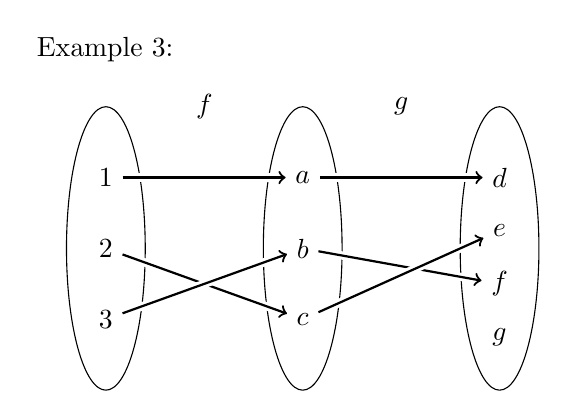
\begin{tikzpicture}[yscale=0.9]
        % sets
            \draw (0,0) ellipse (0.5cm and 2cm);
            \draw (2.5,0) ellipse (0.5cm and 2cm);
            \draw (5,0) ellipse (0.5cm and 2cm);
            \foreach \y/\a/\b/\c in {0/1/a/d,1/2/b/e,2/3/c/f}{
                \node (\a) at (0,1-\y) {\(\a\)}; 
                \node (\b) at (2.5,1-\y) {\(\b\)}; 
                \node (\c) at (5,1-3/4*\y) {\(\c\)}; 
            }
                \node (g) at (5,1-3/4*3) {\(g\)}; 
        % function
            \foreach \a/\b in {1/a,2/c,3/b}{
                \draw[line width=3pt, white] (\a) -- (\b);            
                \draw[->,thick] (\a) -- (\b);
            }
            \foreach \b/\c in {a/d,b/f,c/e}{
                \draw[line width=3pt, white] (\b) -- (\c);            
                \draw[->,thick] (\b) -- (\c);
            }
        % labels
            \node[anchor=south west] at (-1,2.5) {Example 3:};
            \node at (1.25,2) {\(f\)};
            \node at (3.75,2) {\(g\)};
        \end{tikzpicture}\vspace{\baselineskip}
        
        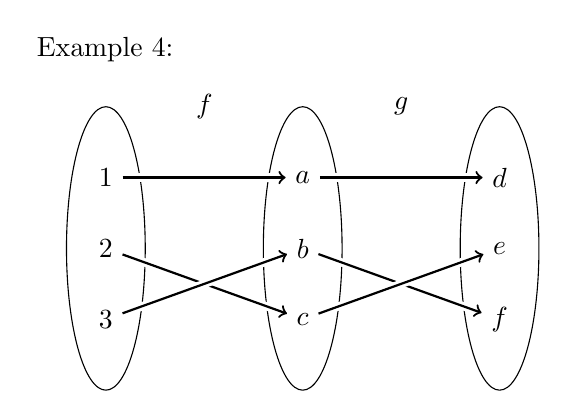
\begin{tikzpicture}[yscale=0.9]
        % sets
            \draw (0,0) ellipse (0.5cm and 2cm);
            \draw (2.5,0) ellipse (0.5cm and 2cm);
            \draw (5,0) ellipse (0.5cm and 2cm);
            \foreach \y/\a/\b/\c in {0/1/a/d,1/2/b/e,2/3/c/f}{
                \node (\a) at (0,1-\y) {\(\a\)}; 
                \node (\b) at (2.5,1-\y) {\(\b\)}; 
                \node (\c) at (5,1-\y) {\(\c\)}; 
            }
        % function
            \foreach \a/\b in {1/a,2/c,3/b}{
                \draw[line width=3pt, white] (\a) -- (\b);            
                \draw[->,thick] (\a) -- (\b);
            }
            \foreach \b/\c in {a/d,b/f,c/e}{
                \draw[line width=3pt, white] (\b) -- (\c);            
                \draw[->,thick] (\b) -- (\c);
            }
        % labels
            \node[anchor=south west] at (-1,2.5) {Example 4:};
            \node at (1.25,2) {\(f\)};
            \node at (3.75,2) {\(g\)};
        \end{tikzpicture}\vspace{\baselineskip}
    \end{tcolorbox}
\end{practice}

\clearpage

\begin{practice}{More Compositions}
    Using \(f(x)=x^2\), \(g(x)=\sqrt{x}\), and \(h(x)=x+1\), find each of the following:
    \begin{enumerate}
        \item \(f\circ h(x)=\)\vspace{3\baselineskip}
        \item \(h\circ f(x)=\)\vspace{3\baselineskip}
        \item \(f\circ g(x)=\)\vspace{3\baselineskip}
        \item \(g\circ f(x)=\)\vspace{3\baselineskip}
    \end{enumerate}
\end{practice}